\documentclass[11pt,a4paper]{scrartcl}
\usepackage[utf8]{inputenc}
\usepackage[utf8]{inputenc}
\usepackage[ngerman]{babel}
\usepackage[T1]{fontenc}
\usepackage{amsmath}
\usepackage{amsfonts}
\usepackage{amssymb}
\usepackage{mathtools}
\usepackage{graphicx}
\usepackage{multirow}
\usepackage{fancyhdr}
\pagestyle{fancy}
\usepackage[a4paper,
			bottom=1.7in,
			left=1.2in,
			right=1.2in,
			top=1.2in,
			headsep = 35pt]
	{geometry}
\usepackage{tikz}% for drawing automata etc
\usetikzlibrary{automata,arrows,chains,shapes.misc,scopes,petri,matrix,patterns}
%\usepackage[x11names]{xcolor}
%\usepackage[parfill]{parskip}
\usepackage{array}
%\usepackage{gslist}
%\usepackage{subfigure}
\usepackage{subcaption}
\usepackage{enumitem}
\usepackage{algpseudocode} %for pseudocode



\setlist[enumerate]{label=\alph*)}
%\setlist[itemize]{label=$\rightarrow$}


 \tikzset{
endbox/.style={pattern=crosshatch,minimum height=.8cm}}

%\partfont{\centering}
\newcommand\tab[1][1cm]{\hspace*{#1}}
\usepackage{framed, color}


\newcommand{\UE}{Übung 1}
\newcommand{\name}{Fragenkatalog zum Überprüfungsgespräch Elektrotechnische Grundlagen}
\title{\textbf{Fragenkatalog zum Überprüfungsgespräch Elektrotechnische Grundlagen Übungen für TI 2017 - \UE}}


\newcommand{\ul}[1]{\underline{#1}} % für unterstreichen von einzelnen Symbolen einfach \ul x - wenn man ein Wort unterstrichen will \ul{wort}
%\newcommand\sy[1]{{\underline{\ifmmode\mathtt{#1}\else\texttt{#1}\fi}}} % ähnlich wie \ul - verwendet aber andere Schriftart
%\newlistt\sys\sy{\hspace{1pt}}{}{}{^} % identisch zu \sy, \sys{wort} unterstreicht aber jeden Buchstaben einzeln und \sy{wort} unterstreicht das ganze Wort
% (sofern das Alphabet nur aus einzelnen Zeichen besteht ist \sys{wort} einfacher


%no line indent
\setlength\parindent{0pt}

\fancyhead[R]{\UE}
\fancyhead[L]{\name}
\fancyfoot[C]{\thepage}

\renewcommand{\footrulewidth}{0pt}
\renewcommand{\headrulewidth}{0.5pt}


\begin{document}
\maketitle

\textbf{Frage 1: Was machst Du gerade im Labor und welchen Sinn hat das?}\\
\textbf{Frage 2: Nenne die Grundgrößen der Elektrotechnik, deren Formelzeichen und Einheit.}\\
Spannung $U[$Volt $V]$, Strom $I[$Ampere $A]$, Widerstand $R[$Ohm $\Omega]$,Leistung $P[$Watt $W]$\\
\textbf{Frage 2: Elektrische Spannung: Nenne Definition (nicht über das Ohmsche Gesetz!), Formelzeichen und Einheit}\\
Die potentielle Energie(=Arbeit) die durch eine Ladungstrennung gespeichert wurde.\\
\textbf{Frage 2: Elektrischer Strom: Nenne Definition (nicht über das Ohmsche Gesetz!), Formelzeichen und Einheit}\\
Ladung eines Elektrons $Q_e=1,6 \cdot 10^{-19}C=1,6 \cdot 10^{-19}A\cdot s$\\
$\frac{6*10^{18}e^-}{1s}=\frac{As}{1s} \rightarrow 6*10^{18}$ Elektronen fließen durch einen Leiter pro Sekunde bei $1A$\\
\textbf{Frage 2: Elektrischer Widerstand: Nenne Definition (nicht über das Ohmsche Gesetz!), Formelzeichen und Einheit}\\
Ist eine Materialeigenschaft\\
Beispiel Kupfer $17m\Omega \cdot mm^2/m$\\
\textbf{Frage 2: Elektrische Leistung: Nenne Definition, Formelzeichen und Einheit}\\
Die in einer Zeitspannung umgesetzte elektrische Energie bezogen auf die Zeitspanne.\\
\textbf{Frage 2: Wie berechnet man die elektrische Leistung in einem Gleichstromkreis?}\\
$U=R \cdot I \rightarrow P=U \cdot I$\\
\textbf{Berechne die an einem Widerstand entstehende Leistung, wenn durch ihn bei einer Spannung von $2V$ ein Strom von $3A$ fließt.}\\
$6W$\\
\textbf{Frage 2: Welcher Phasenwinkel besteht zwischen Wechselspannung und Wechselstrom an einem idealen Kondensator?}\\
Die Spannung folgt dem Strom um $90^\circ=\pi/2$ nach. (eigentlich $-90^\circ$)\\
\textbf{Welcher Phasenwinkel besteht zwischen Wechselspannung und Wechselstrom an einer idealen Induktivität?\\
(Die Vorzeichen brauchen nicht explizit angegeben zu werden, müssen aber verglichen werden).}\\
Der Strom folgt der Spannung nach um $90^\circ=\pi/2$ nach. (eigentlich $+90^\circ$)\\
\textit{Gehen in entgegengesetzte Richtungen!}\\
\textbf{Frage 2: Formuliere das ohmsche Gesetz.}\\
$U=R*I$\\
\textbf{Berechne den Widerstand, wenn bei einem Strom von $3A$ eine Spannung von $3V$ abfällt.}\\
\textbf{Frage 2: Berechne den Strom, wenn an einem Widerstand von $5\Omega$ eine Spannung von $10V$ abfällt.}\\
\textbf{Frage 2: Berechne die Spannung, wenn durch einen Widerstand von $10\Omega$ ein Strom von $5A$ fließt. }\\
\textbf{Frage 2: Formuliere die Kirchhoffschen Regeln.}\\
\textbf{Auf welchem physikalischen Grundprinzip beruhen diese?}\\
\textit{Energieerhaltung}\\
Maschenregel: Summe aller Spannungen muss 0 ergeben.\\
Knotenregel: Summe aller Ströme muss 0 ergeben.\\
\textbf{An einem Spannungsteiler liegen $9V$. Am oberen Widerstand liegen $6V$ an.}\\
\textbf{Berechne die Spannung am unteren Widerstand.}\\
\textbf{Frage 2: In einen Stromknoten mit drei Leitungen fließen aus einer Leitung $2A$ hinein und aus einer anderen Leitung $3A$ hinein. Was geschieht in der dritten Leitung?}\\
\textbf{Frage 2: Nenne die Zehnerpotenzen zu den SI - Präfixen Nano, Milli und Mikro. Nenne die SI - Präfixe zu: $10^3, 10^6, 10^9$}\\
\begin{tabular}{|l|l|l|}
\hline
\textbf{Präfix} & \textbf{Zeichen} & \textbf{Faktor}\\
\hline\hline
Piko   & p  & $10^{-12}$\\
\hline
Nano   & n  & $10^{-9}$\\
\hline
Mikro  & $\mu$ & $10^{-6}$\\
\hline
Milli  & m  & $10^{-3}$\\
\hline
Zenti  & c  & $10^{-2}$\\
\hline
Dezi   & d  & $10^{-1}$\\
\hline\hline
Deka   & da & $10^{1}$\\
\hline
Hekto  & h  & $10^{2}$\\
\hline
Kilo   & k  & $10^{3}$\\
\hline
Mega   & M  & $10^{6}$\\
\hline
Giga   & G  & $10^{9}$\\
\hline
Tera   & T  & $10^{12}$\\
\hline
\end{tabular}\\
\textbf{Frage 3: Benenne die beiden wichtigsten elektrotechnischen Eigenschaften (Größen) eines Widerstandes (konkreter Bauteil) und gib die korrekten Einheiten dazu an.}\\
Widerstand $R[$Ohm $\Omega]$, \textit{Leitwert}$=\frac{1}{R}$, Maximalleistung $P_{MAX}[$Watt $W]$\\
\textbf{Benenne die wichtigste elektrotechnische Eigenschaft (Größe) eines Kondensators (konkreter Bauteil) und gib die korrekte Einheit dazu an.}\\
Kapazität $[$Farad $F]$\\
\textbf{Benenne die wichtigste elektrotechnische Eigenschaft (Größe) einer Spule (konkreter Bauteil) und gib die korrekte Einheit dazu an.}\\
Induktivität $[$Henry $H]$\\
\textbf{Frage 3: Wie ist ein Spannungsmessgerät mit einer Schaltung zu verbinden?}\\
Spannungsrichtig $=$ Paralell\\
\textbf{Wie ist ein Strommessgerät mit einer Schaltung zu verbinden?}\\
Stromrichtig $=$ Seriell\\
\textbf{Welche Maßnahme ist logischerweise nach Abschluss einer Strommessung notwendig?}\\
Schließen des Stromkreises\\
\textbf{Frage 3: Was ist eine Kennlinie?}\\
Darstellung des Stroms in Abhängigkeit der Spannung\\
\textbf{Skizziere die Kennlinie eines ohmschen Widerstandes.}\\
linear\\
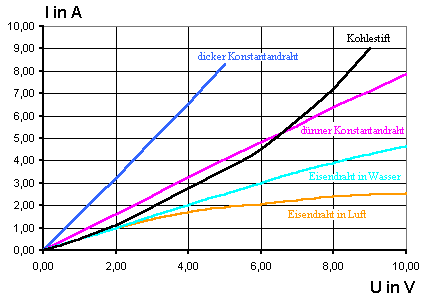
\includegraphics[height=6cm,keepaspectratio]{Kennlinie_Ohm.png}\\
\textbf{Skizziere die Kennlinie einer Diode.}\\
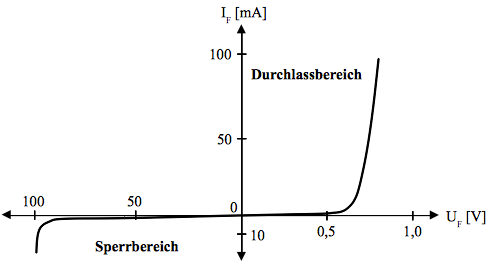
\includegraphics[height=6cm,keepaspectratio]{Kennlinie_Diode.png}\\
\textbf{Frage 3: Nenne die drei Kenngrößen sinusförmiger gleichspannungsfreier Wechselspannung!\\
Benenne auch die korrekten Einheiten dazu!}\\
Amplitude $[V]$, Frequenz $[Hz]$, Phase $[rad$ oder $deg]$\\
\textbf{Frage 4: Es gibt drei Arten der Messung von Widerstandswerten. Benenne und beschreibe sie (Schaltskizze).}
\begin{enumerate}
	\item Direkte Messung mit Ohmmeter (Multimeter).
	\item Indirekte Messung durch Strommessung. (Stromrichtig)
	\item Indirekte Messung durch Spannungsmessung. (Spannungsrichtig)
\end{enumerate}
\textbf{Frage 4: Ein Spannungsteiler $1k\Omega$ zu $3k\Omega$ liegt an einer Spannung von $8V$. Skizziere die Schaltung und berechne die Spannungen an den beiden Widerständen.}\\
Spannungsverhältnis = Widerstandsverhältnis\\
$U_1=2V$,$U_2=6V$\\
\textbf{Frage 4: Ein Spannungsteiler $1k\Omega$ zu $2k\Omega$ parallel $2k\Omega$ liegt an einer Spannung von $8V$. Skizziere die Schaltung und berechne die beiden Teilspannungen.}\\
Zuerst Paralellschaltung zusammenfassen\\
\textbf{Frage 4: Berechne die unbekannte Spannung in folgender Schaltung: Welches Prinzip verwendest Du dabei? (2 Antworten zulässig.)}\\
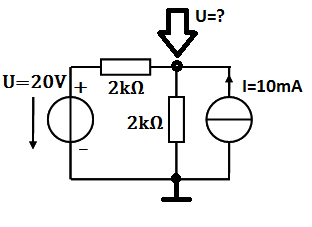
\includegraphics[height=6cm,keepaspectratio]{Spannung_berechnen.png}\\
Superpositionsprinzip oder Knoten und Maschenregel $U=20V$\\
\textbf{Frage 4: Berechne den unbekannten Strom in folgender Schaltung: Welches Prinzip verwendest Du dabei? (2 Antworten zulässig.)}\\
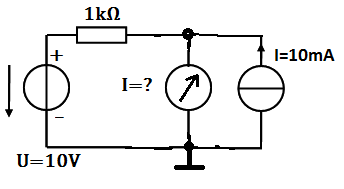
\includegraphics[height=6cm,keepaspectratio]{Strom_berechnen.png}\\
\textit{Mitte ideales Strommessgerät.}\\
Superpositionsprinzip oder linker und rechter Kreis einzeln, da Strommessgerät $R_innen=unendlich$. $I=10mA+10mA=20mA$\\
\textbf{Frage 5: Was ist ein Oszilloskop?}\\
Ein Gerät zur Messung einer Spannung über einen Zeitverlauf.\\
\textbf{Frage 5: Benenne die beiden wichtigsten Bedienungselemente des Oszilloskops für die Y - Achse.}\\
\begin{itemize}
	\item Einstellung der Höhe der Nulllinie
	\item Einstellung der Skalierung der Y-Achse (Damit Maximalwert \& Minimalwert angezeigt werden kann)
\end{itemize}
\textbf{Beschreibe die Methode der Amplitudenmessung mit dem Oszilloskop gemäß Bild.}\\
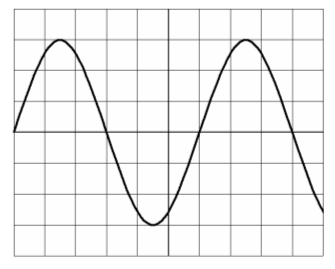
\includegraphics[height=3cm,keepaspectratio]{Oszi.png}\\
Die Amplitude ist $1V/DIV$ (=Skalaabschnitt) $\rightarrow$ Maximale Amplitude $8V$. Amplitude auf Skizze $3V$ bzw $-3V$.\\
\textbf{Frage 5: Benenne die beiden wichtigsten Bedienungselemente des Oszilloskops für die X - Achse.}\\
\begin{itemize}
	\item Verschiebung in horizontaler Richtung (Offset)
	\item Einstellung der Skalierung der X-Achse (Damit das Zeitfenster das betrachtet wird vollständig angezeigt wird)
\end{itemize}
\textbf{Beschreibe die Methode der Periodenzeitmessung mit dem Oszilloskop gemäß Bild.}\\
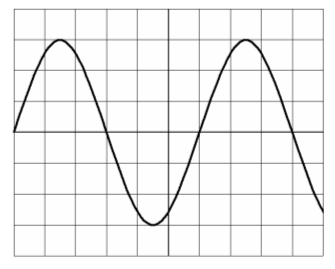
\includegraphics[height=3cm,keepaspectratio]{Oszi.png}\\
Die Amplitude ist 1ms/DIV (=Skalaabschnitt) $\rightarrow$ Angezeigtes Zeitintervall $10ms$. Periodenzeit auf Skizze $6ms$.\\
\textbf{Frage 5: Beschreibe Zweck, elementare Bedienungselemente und elementare Bedienung der Trigger - Einheit des Oszilloskops.}
\begin{itemize}
	\item Für jeden Kanal $V/DIV$ für Skalierung der Amplitude
	\item Skalierung Zeitachse $ms/DIV$
	\item Trigger Regler (zB.: welcher Eingang \emph{Trigger Quelle}, Spannungswert überschritten \emph{Trigger Level}, steigende/fallende Flanke \emph{Trigger Richtung}) - Signal gut darstellen
\end{itemize}
\textbf{Frage 5: Wozu dient ein Funktionsgenerator?}\\
Erzeugen einer Spannung die sich \textit{periodisch} über die Zeit ändert. zB.: Sinus-, Rechteck-, Dreieck-, Sägezahnimpulse.\\
\textbf{Nenne drei wichtige Einstellungen eines Funktionsgenerators.}
\begin{itemize}
	\item Frequenz
	\item Amplitude
	\item Symmetrie
	\item Gleichanteil (=linearer zeitlicher Mittelwert)
\end{itemize}
\textbf{Frage 5: Benenne drei wichtige vom Funktionsgenerator gelieferte Signalformen auf Deutsch und Englisch und skizziere diese.}\\
		\begin{minipage}{0.49\linewidth} 
      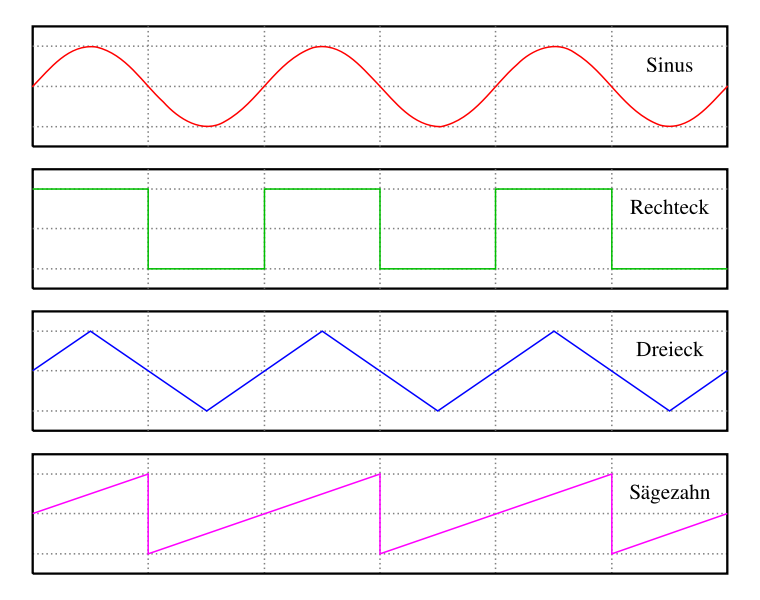
\includegraphics[height=6cm,keepaspectratio]{Funktionsgenerator_Wellenformen.png}
    \end{minipage} 
    \hfill 
    \begin{minipage}{0.49\linewidth} 
      \begin{itemize}
				\item Sinus = Sine
				\item Rechteck = Square
				\item Dreieck = Triangle
				\item Sägezahn = \textit{Ramp}
			\end{itemize}
    \end{minipage} \\
\textbf{Frage 5: Was ist der Unterschied zwischen Y - T und X - Y Betrieb eines Oszilloskops?}
\begin{itemize}
	\item Y - T: \textit{Zeitbereich} Signal am X Eingang in abhängigkeit der Zeit $\rightarrow$ muss Funktion sein!
	\item X - Y: \textit{Bildbereich} Signal am X Eingang in abhängigkeit von Y $\rightarrow$ Lissajous Funktion für Frequenz- \& Phasenwinkelbestimmung
\end{itemize}
\textbf{Frage 5: Warum muss in dieser Schaltung Kanal Y1 des Oszilloskops invertiert geschalten werden?}\\
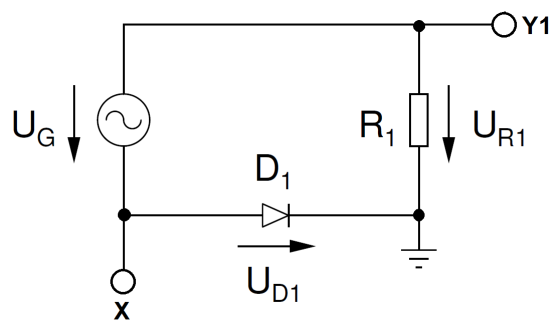
\includegraphics[height=6cm,keepaspectratio]{Oszi_Schaltung.png}\\
\textit{Sinusförmige Wechselspannungsquelle}\\
Masse des Oszilloskop immer mit Erde verbunden!\\
Y1 invertiert weil an X eine negative Spannung anliegt, da sich die Schaltung sonst verändern würde.\\
Positiver Strom nach der Diode ergibt negative Spannung am Widerstand wegen position der Masse. Masse gibt Nullpunkt an!\\
\textbf{Warum darf bei solchen Aufbauten die Masse des Funktionsgenerators nicht mit Erde verbunden sein?}\\
Da sonst eine Kurzschlussverbindung zwischen der Masse des Funktionsgenerators und der Schutzmasse entsteht!\\
\textbf{Frage 5: Die Werte des Widerstandes, des Kondensators und der Frequenz werden so gewählt, dass die Amplituden der Spannungen X und Y1 gleich sind. Die Wechselspannung ist sinusförmig. Das Oszilloskop ist in Betriebsart X-Y geschalten. Welche Kurve zeigt das Oszilloskop? Wie kann man diese Kurve mathematisch erklären?}\\
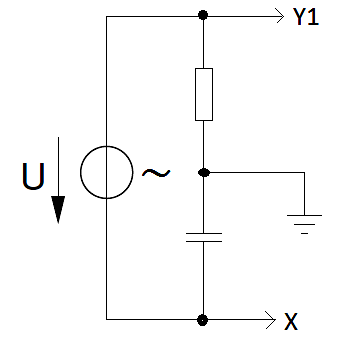
\includegraphics[height=6cm,keepaspectratio]{Oszi_Widerstand.png}\\
Lissajousfigur (Kreis) da Frequenzen gleich sind.\\
$x=A \cdot cos(t)$,$y=A \cdot sin(t)$ ($A$ = Amplitude der Schwingungen bzw Radius des Kreises, wenn unterschiedlich dann Ellipse)\\
\end{document}
